
%(BEGIN_QUESTION)
% Copyright 2007, Tony R. Kuphaldt, released under the Creative Commons Attribution License (v 1.0)
% This means you may do almost anything with this work of mine, so long as you give me proper credit

Here is a pneumatic P+I controller mechanism, with reset (integral) action implemented in the standard way:

$$\includegraphics[width=15.5cm]{i01610x02.eps}$$

\filbreak

This is called ``internal reset'' action.  There is, however, an alternative method for implementing reset action in a pneumatic controller, and it involves the addition of a pneumatic position transmitter on the valve to signal valve stem position to the controller.  This alternative method is called ``external reset:''

$$\includegraphics[width=15.5cm]{i01610x01.eps}$$

The benefit of a controller with external reset is that the reset action has less of a tendency to ``wind up.''  Explain why this is.

\vskip 10pt

Hint: imagine the valve is equipped with a minimum-travel ``stop'' so that its furthest-closed position is 15\%.  Stops are sometimes used on flow-control valves where a certain minimum flow rate must be maintained for process safety reasons (e.g. flow control for process fluid in a combustion heater where zero flow might result in overheated and ruptured tubes).  How would external reset help prevent the controller from winding down under certain low-setpoint conditions?

\vskip 20pt \vbox{\hrule \hbox{\strut \vrule{} {\bf Suggestions for Socratic discussion} \vrule} \hrule}

\begin{itemize}
\item{} A powerful problem-solving technique is performing a {\it thought experiment} where you mentally simulate the response of a system to some imagined set of conditions.  Describe a useful ``thought experiment'' for this system, and how the results of that thought experiment are helpful to answering the question.  If you find this system too complex, apply another problem-solving technique: {\it simplify} the system, then analyze the simpler system.
\item{} How would this external reset scheme work on a control valve with really bad hysteresis (stiction)?  Would the loop ``cycle'' as a normal internal-reset controller driving a sticky valve would exhibit a stick-slip cycle, or not?
\item{} Identify how you could increase the gain of this controller without moving the fulcrum.
\end{itemize}

\underbar{file i01610}
%(END_QUESTION)





%(BEGIN_ANSWER)

External anti-reset windup is a feature available on some controllers for preventing ``windup'' of the integral (reset) term, by monitoring valve position or some other real-world indication of output saturation.  It works by stopping integration whenever the actual final control element is saturated, rather than stopping integration based on a maximum or minimum set value programmed into the controller.

\vskip 10pt

With integral action based on valve position rather than the controller's output signal magnitude, windup will be prevented over a wider range of conditions.  For instance, if the valve were to become jammed or limited in travel by a ``stop,'' integration would cease at that limit, rather than blindly progress until the actual controller output pressure reached saturation as would be the case with internal anti-reset windup.

This will not prevent all cases of reset windup, but it will help the controller recover from incidents of windup resulting from valve position saturation.

\vskip 10pt

Interestingly, this very same technique is used in FOUNDATION Fieldbus PID loops, where the analog output function block provides a ``back calculation'' signal (BKCAL\_OUT) for the input of the PID block.  If the final control element cannot attain a certain state, for whatever reason, the PID block will know this and cease integrating, thus preventing needless windup:

$$\includegraphics[width=15.5cm]{i01610x03.eps}$$

%(END_ANSWER)





%(BEGIN_NOTES)


%INDEX% Control, integral: external reset
%INDEX% Control, integral: windup mitigation through external reset

%(END_NOTES)


